%\documentclass[handout]{beamer}
%\documentclass{beamer}
\documentclass[aspectratio=169]{beamer}

\mode<presentation>
{
  \usetheme[hideothersubsections]{Goettingen}
  \usecolortheme{beaver}
}

\usepackage{fontenc}
\usepackage{multirow}
\usepackage{multicol}
\usepackage[export]{adjustbox}
\usepackage{listings}
\usepackage{pgf, pgffor}
\usepackage{lstlinebgrd} % see http://www.ctan.org/pkg/lstaddons
\usepackage{caption}
\usepackage{graphicx}
\usepackage{pifont}% http://ctan.org/pkg/pifont
\usepackage{xcolor,colortbl}
\usepackage{hyperref}
%\usepackage{pgfplots}
\usepackage{tcolorbox}
\usepackage{pgfpages}
\usepackage{savesym}
\usepackage{amsmath}
\savesymbol{checkmark}

\usepackage{dingbat}

\title[The Art of Writing Reasonable Concurrent Code]{The Art of Writing Reasonable Concurrent Code\\ {\small Pre-Conference Workshop ACCU 2017} \\ {\footnotesize \copyright 2017}}
\author{Felix Petriconi}
\date{2017-04-25}

% -----------------------------------------------------------------------------------------
% custom makros
% -----------------------------------------------------------------------------------------
\newcommand{\cppkey}[1]{\texttt{\textcolor{blue}{#1}}}
\newcommand{\cmark}{\textcolor{green}{\ding{51}}}
\newcommand{\xmark}{\textcolor{red}{\ding{55}}}
\newcommand{\outputbox}[1]{%
	\begin{tcolorbox}[colback=gray!5,colframe=gray!40!black,title=Output]%
		\begin{flushleft}%
			{\tiny #1}%
		\end{flushleft}%
	\end{tcolorbox}%
}
% -----------------------------------------------------------------------------------------

\definecolor{mygreen}{rgb}{0,0.6,0}
\definecolor{mygray}{rgb}{0.5,0.5,0.5}
\definecolor{mymauve}{rgb}{0.58,0,0.82}
\definecolor{columnheadinggray}{rgb}{0.6,0.6,0.6}

\lstset{ %
  backgroundcolor=\color{white},   % choose the background color; you must add \usepackage{color} or \usepackage{xcolor}
  basicstyle=\ttfamily\tiny,       % the size of the fonts that are used for the code
  breakatwhitespace=false,         % sets if automatic breaks should only happen at whitespace
  breaklines=true,                 % sets automatic line breaking
  captionpos=none,                   % sets the caption-position to top
  commentstyle=\color{mygreen},      % comment style
  deletekeywords={...},            % if you want to delete keywords from the given language
  escapeinside={/*}{*/},           % if you want to add LaTeX within your code
  extendedchars=true,              % lets you use non-ASCII characters; for 8-bits encodings only, does not work with UTF-8
  frame=single,	                   % adds a frame around the code
  keepspaces=true,                 % keeps spaces in text, useful for keeping indentation of code (possibly needs columns=flexible)
  keywordstyle=\color{blue},       % keyword style
  language=C++,                    % the language of the code
  otherkeywords={alignas,alignof,
    char16_t,char32_t,constexpr,
    decltype,declval,noexcept,
    nullptr,static_assert,
    thread_local,override,final}, % if you want to add more keywords to the set
  numbers=left,                    % where to put the line-numbers; possible values are (none, left, right)
  numbersep=5pt,                   % how far the line-numbers are from the code
  numberstyle=\tiny\color{mygray}, % the style that is used for the line-numbers
  rulecolor=\color{black},         % if not set, the frame-color may be changed on line-breaks within not-black text (e.g. comments (green here))
  showspaces=false,                % show spaces everywhere adding particular underscores; it overrides 'showstringspaces'
  showstringspaces=false,          % underline spaces within strings only
  showtabs=false,                  % show tabs within strings adding particular underscores
  stepnumber=1,                    % the step between two line-numbers. If it's 1, each line will be numbered
  stringstyle=\color{mymauve},     % string literal style
  tabsize=2,	                   % sets default tabsize to 2 spaces
  title=\lstname                   % show the filename of files included with \lstinputlisting; also try caption instead of title
}

\lstdefinestyle{CodeInTextStyle} {
    basicstyle=\ttfamily\normalsize,
    frame=none,
    numbers=none,
    captionpos=none
}

\DeclareCaptionFont{white}{\color{white}}
\DeclareCaptionFormat{listing}{\noindent\colorbox{gray}{\parbox{\linewidth}{#1#2#3}}}
\captionsetup[lstlisting]{format=listing,labelfont=white,textfont=white, font=scriptsize}

%=====================================================================================================
% Define background box capabilities for source code listings
% Taken from http://tex.stackexchange.com/questions/8851/how-can-i-highlight-some-lines-from-source-code?lq=1
%=====================================================================================================

\makeatletter
%%%%%%%%%%%%%%%%%%%%%%%%%%%%%%%%%%%%%%%%%%%%%%%%%%%%%%%%%%%%%%%%%%%%%%%%%%%%%%
%
% \btIfInRange{number}{range list}{TRUE}{FALSE}
%
% Test in int number <number> is element of a (comma separated) list of ranges
% (such as: {1,3-5,7,10-12,14}) and processes <TRUE> or <FALSE> respectively

\newcount\bt@rangea
\newcount\bt@rangeb

\newcommand\btIfInRange[2]{%
    \global\let\bt@inrange\@secondoftwo%
    \edef\bt@rangelist{#2}%
    \foreach \range in \bt@rangelist {%
        \afterassignment\bt@getrangeb%
        \bt@rangea=0\range\relax%
        \pgfmathtruncatemacro\result{ ( #1 >= \bt@rangea) && (#1 <= \bt@rangeb) }%
        \ifnum\result=1\relax%
            \breakforeach%
            \global\let\bt@inrange\@firstoftwo%
        \fi%
    }%
    \bt@inrange%
}
\newcommand\bt@getrangeb{%
    \@ifnextchar\relax%
        {\bt@rangeb=\bt@rangea}%
        {\@getrangeb}%
}
\def\@getrangeb-#1\relax{%
    \ifx\relax#1\relax%
        \bt@rangeb=100000%   \maxdimen is too large for pgfmath
    \else%
        \bt@rangeb=#1\relax%
    \fi%
}

%%%%%%%%%%%%%%%%%%%%%%%%%%%%%%%%%%%%%%%%%%%%%%%%%%%%%%%%%%%%%%%%%%%%%%%%%%%%%%
%
% \btLstHL<overlay spec>{range list}
%
% TODO BUG: \btLstHL commands can not yet be accumulated if more than one overlay spec match.
%
\newcommand<>{\btLstHL}[1]{%
  \only#2{\btIfInRange{\value{lstnumber}}{#1}{\color{orange!30}\def\lst@linebgrdcmd{\color@block}}{\def\lst@linebgrdcmd####1####2####3{}}}%
}%
\makeatother

%=====================================================================================================

%\AtBeginSection[]{ % Do nothing for \section*
%	\setbeamercolor{section in toc}{fg=black}
%	\setbeamercolor{subsection in toc}{fg=black}
%	\begin{frame}<beamer>
%        \frametitle{Outline \insertsectionhead}
%		\tableofcontents[hidesubsections]
%	\end{frame}
%}

\setbeamertemplate{footline}[frame number]

\begin{document}
\beamertemplatenavigationsymbolsempty

%=====================================================================================================
%=====================================================================================================
%=====================================================================================================

\begin{frame}
    \titlepage
    \begin{center}
    \url{git@github.com:FelixPetriconi/accu2017_course.git}
    \end{center}
\end{frame}

%=====================================================================================================
%=====================================================================================================
%=====================================================================================================


\begin{frame}{}
	\begin{center}
	    The [C++] language is too large for \textit{anyone} to master\\
	    \pause
	    So \textit{everyone} lives within a subset\\
	    \pause
	\end{center}
	\begin{flushright}
	    {\small \textit{Sean Parent, C++Now, 2012}}
	\end{flushright}
\end{frame}


%=====================================================================================================
%=====================================================================================================
%=====================================================================================================


\part{Why are were here?}


\begin{frame}{Felix Petriconi}
	\begin{itemize}
	    \item School (UCSD Pascal, Turbo Pascal)
		\item Studied electrical engineering (Modula 2, Ada, C++)
		\item Student research assistant (1992-1996) (Turbo Pascal, C++, C)
		\item Freelance programmer 1996-2003 (Ericsson, Siemens-VDO, etc.)
			\begin{itemize}
				\item Development of test software for embedded devices (Perl, C)
			\end{itemize}
		\item Programmer and development manager 2003-today at MeVis Medical Solutions AG, Bremen, Germany
		\begin{itemize}
			\item Development of medical devices in the area of mammography and radio therapy (C++, Ruby, Python)
		\end{itemize}
		\item Programming activities:
			\begin{itemize}
				\item Blog editor of ISO C++ website
				\item Active member of C++ User Group Bremen
				\item Contributor to Sean Parent's concurrency library
				\item Member of ACCU conference committee
			\end{itemize}
		\item Married with Nicole, having three children, living near Bremen, Germany
		\item Other interests: Classic film scores, composition
	\end{itemize}
\end{frame}


\begin{frame}<handout:0>
	\begin{center}
	Why are we here?
	\end{center}
\end{frame}


\section{Why am I here?}

\begin{frame}{Why am I here?}
  \pause
	I saw how we developed multi threaded code in the past.\\
	I saw how easy it is to make mistakes.\\
	I saw and still see how difficult it is to maintain this code.\\
	\medskip \pause
	I watched recordings from Sean Parent's talks about  "Better Code".\\
	I was impressed.\\
	I wanted to learn more.\\
	\medskip \pause
	I'm collaborating in his open source project for a new library.\\
	I'm continuously learning there a lot.\\
	I care about sharing my knowledge, here at the ACCU conference.
\end{frame}


\section{Why are you here?}


\begin{frame}{Why are you here?}
	\begin{center}
		What is your motivation to be here?
	\end{center}
\end{frame}


\section{Motivation}


\subsection{Problems from my domain}

\begin{frame}{Problems from my domain}
	\begin{itemize}
		\item Loading of huge images blocks UI
		\item Storing of files blocks UI
		\item Re-coding of huge images takes very long
		\item DB accesses takes too long
		\item ...
	\end{itemize}	
\end{frame}



\begin{frame}
    \begin{center}
    Why do we have to talk about concurrency?
    \end{center}
\end{frame}



\begin{frame}{}
	\begin{center}
	    The free lunch is over!
	\end{center}
	\pause
	\begin{flushright}
		\textit{Herb Sutter, 2005}\footnotemark
	\end{flushright}
	\pause
	\only<3->{\footnotetext[1]{The Free Lunch Is Over: A Fundamental Turn Toward Concurrency in Software \url{http://www.gotw.ca/publications/concurrency-ddj.htm}} }

\end{frame}


\begin{frame}{The free lunch is over}
    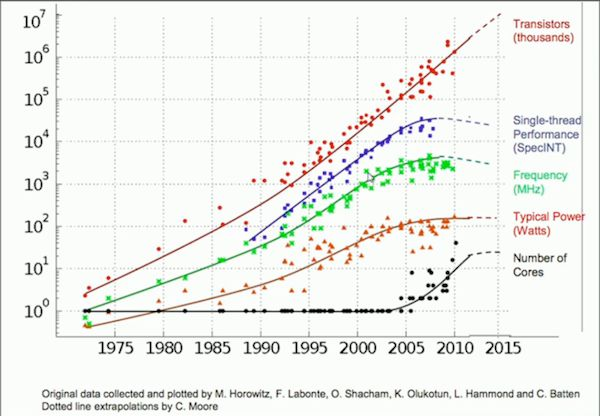
\includegraphics[width=0.8\textwidth]{Introduction/TheFreeLunchIsOver.jpg}
\end{frame}


\begin{frame}<handout:0>{Desktop Compute Power}
    8-core 3.5GHz (Sandy Bridge + AMD Radeon 6950)
    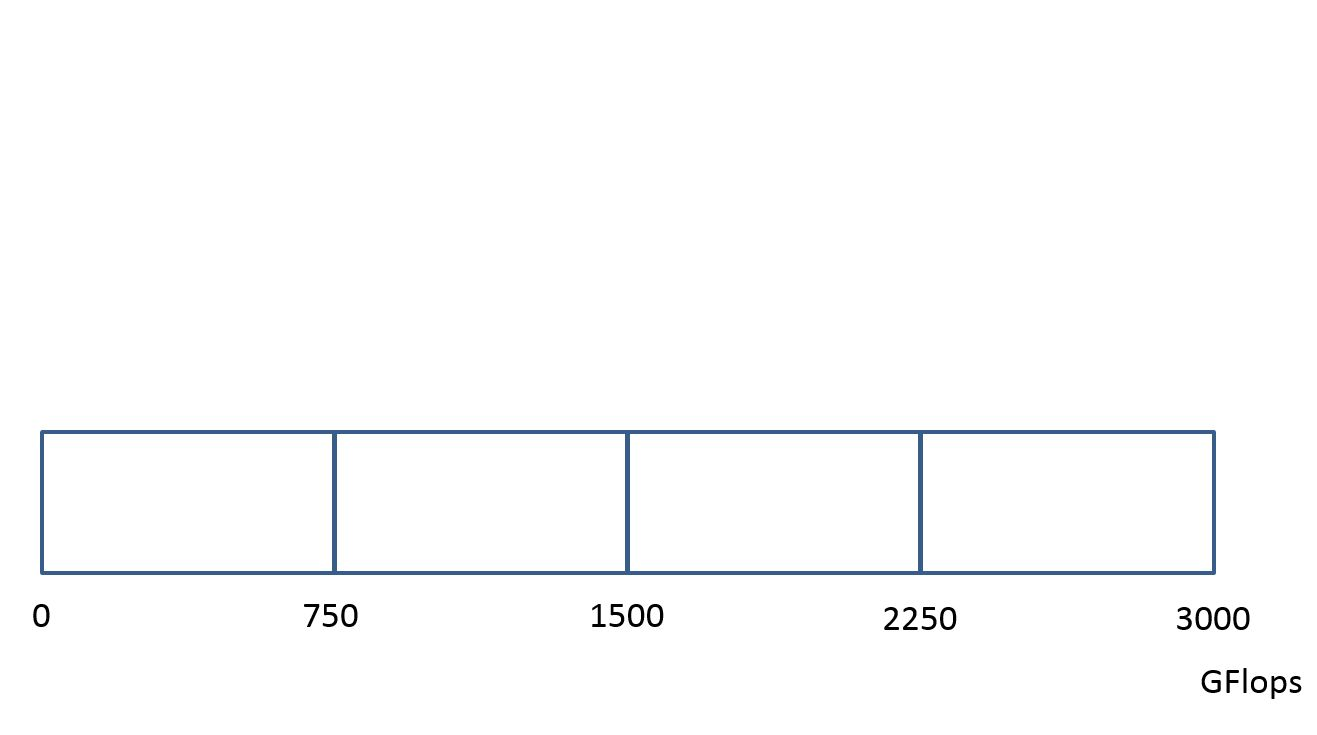
\includegraphics[width=\textwidth]{Introduction/DesktopComputePower01.jpg}
\end{frame}

\begin{frame}<handout:0>{Desktop Compute Power}
    8-core 3.5GHz (Sandy Bridge + AMD Radeon 6950)
    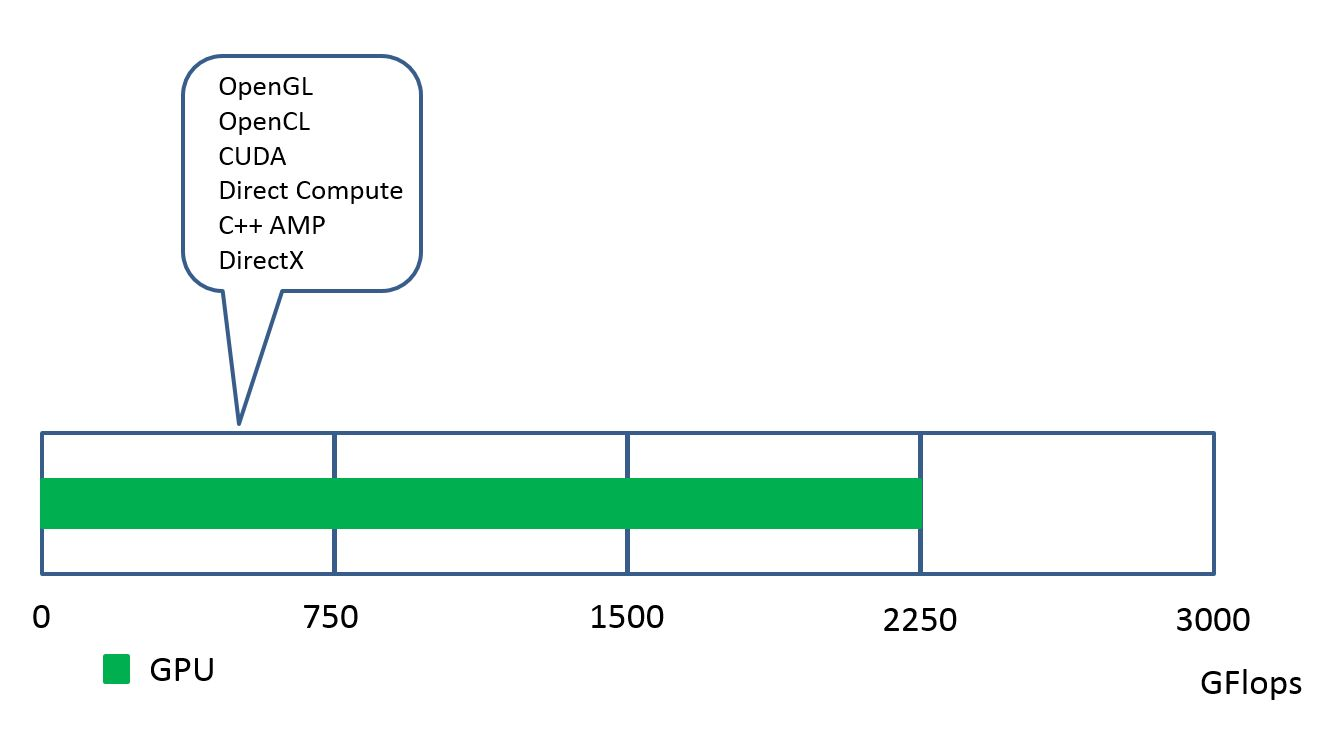
\includegraphics[width=\textwidth]{Introduction/DesktopComputePower02.jpg}
\end{frame}

\begin{frame}<handout:0>{Desktop Compute Power}
    8-core 3.5GHz (Sandy Bridge + AMD Radeon 6950)
    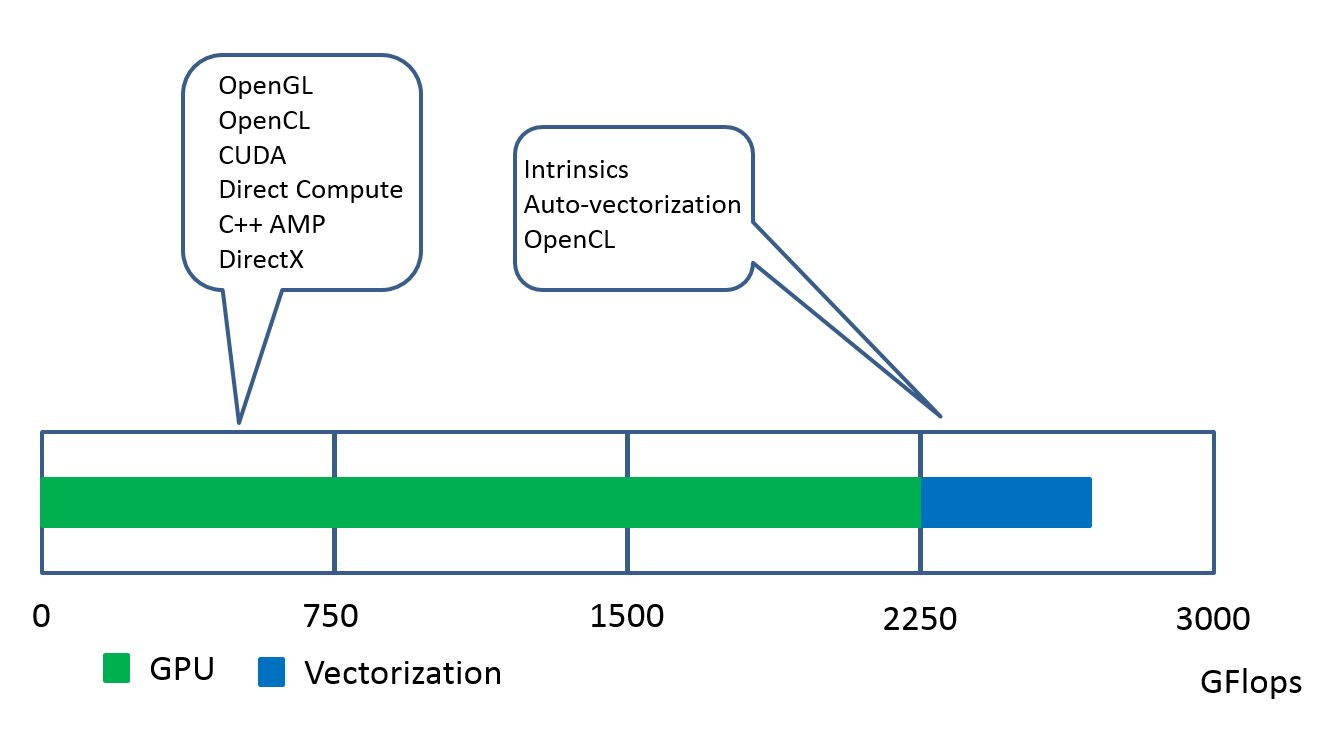
\includegraphics[width=\textwidth]{Introduction/DesktopComputePower03.jpg}
\end{frame}

\begin{frame}<handout:0>{Desktop Compute Power}
    8-core 3.5GHz (Sandy Bridge + AMD Radeon 6950)
    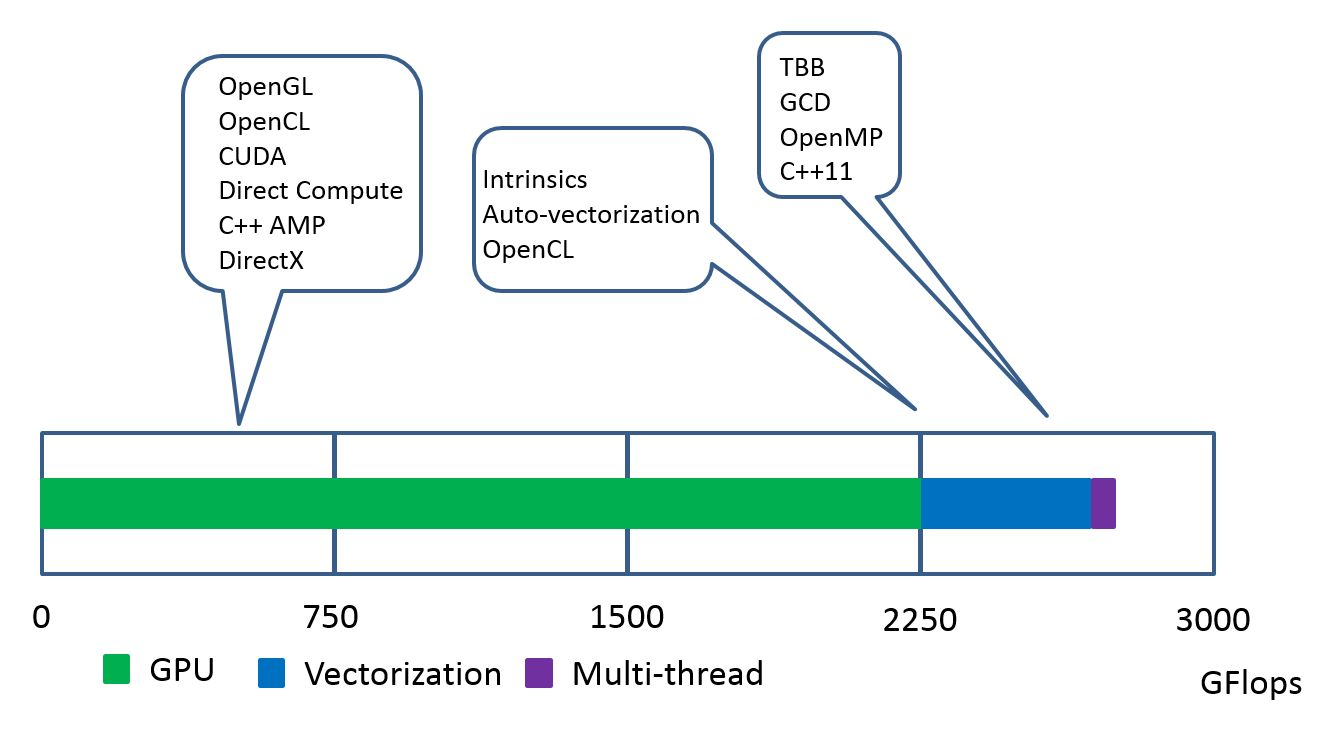
\includegraphics[width=\textwidth]{Introduction/DesktopComputePower04.jpg}
\end{frame}

\begin{frame}<handout:0>{Desktop Compute Power}
    8-core 3.5GHz (Sandy Bridge + AMD Radeon 6950)
    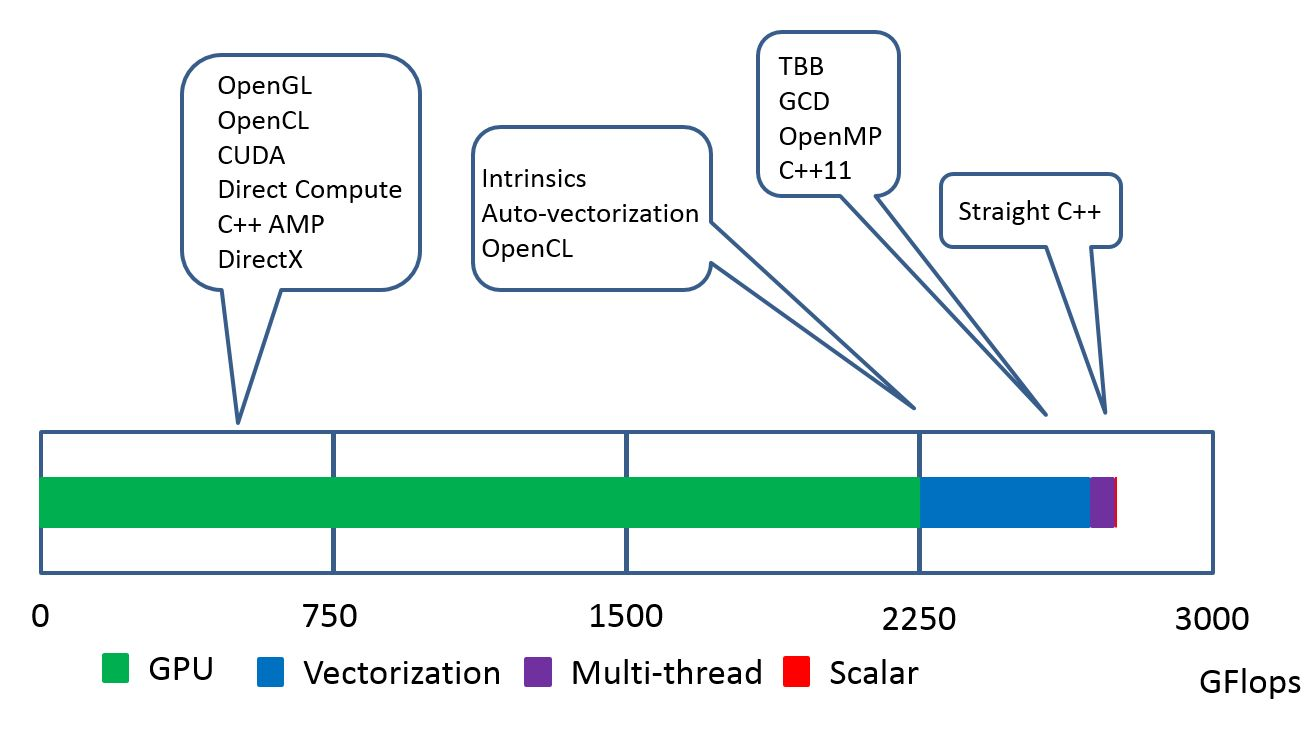
\includegraphics[width=\textwidth]{Introduction/DesktopComputePower05.jpg}
\end{frame}

\begin{frame}{Desktop Compute Power}
    8-core 3.5GHz (Sandy Bridge + AMD Radeon 6950)
    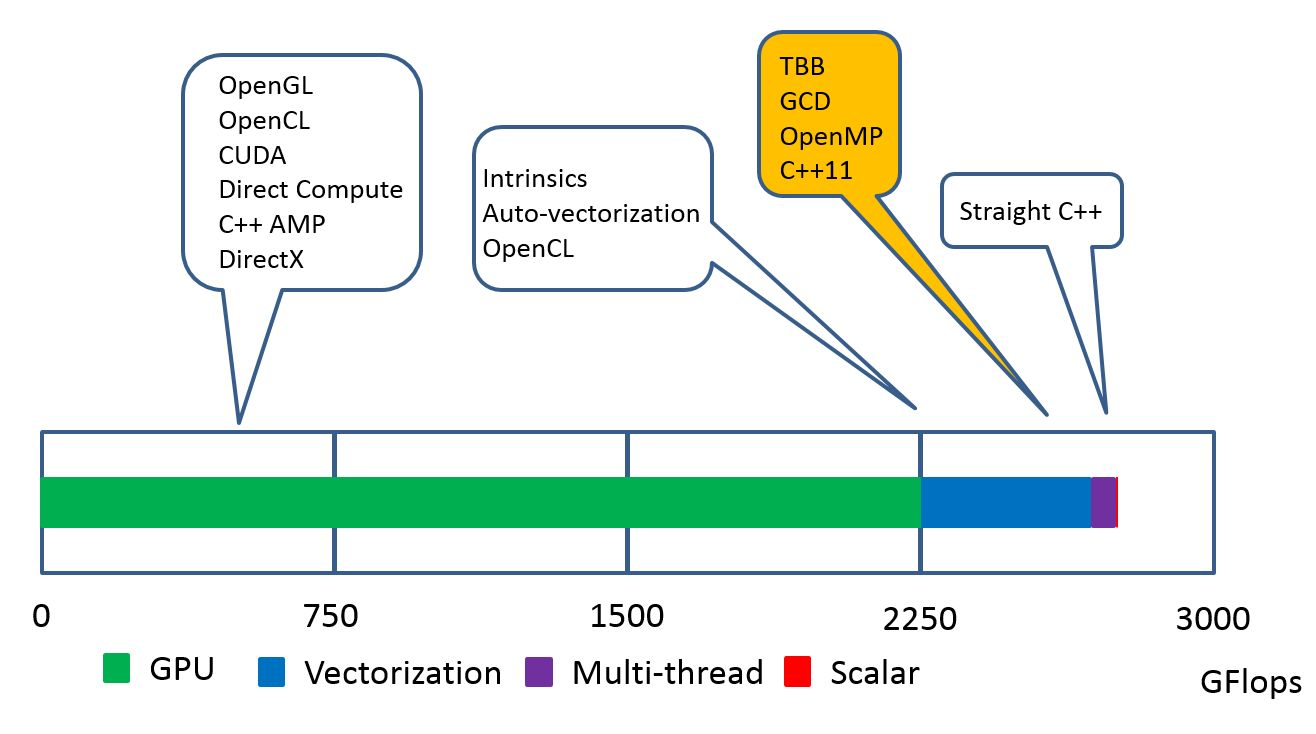
\includegraphics[width=\textwidth]{Introduction/DesktopComputePower06.jpg}
    \linebreak
    That's what we are targeting for!
\end{frame}


\begin{frame}<handout:0>{Amdahl's Law}
	\begin{columns}
		\begin{column}{0.25\textwidth}
			$S(N) = \frac{1}{(1-P)+\frac{P}{N}}$\\
			\begin{tabular}{ll}
				$P:$ & {\small Synchronization $[0 - 1]$} \\
				$N:$ & {\small Number of Cores}\\
			\end{tabular}
		\end{column}
		\begin{column}{0.75\textwidth}
		\end{column}
	\end{columns}
\end{frame}


\begin{frame}{Amdahl's Law}
	0\% Synchronization
	\begin{columns}
		\begin{column}{0.25\textwidth}
		   $S(N) = \frac{1}{(1-P)+\frac{P}{N}}$\\
		   $P = 0$
		\end{column}
		\begin{column}{0.75\textwidth}
		     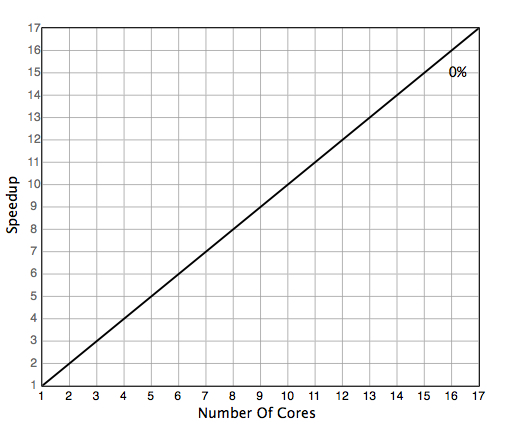
\includegraphics[width=0.75\textwidth]{Introduction/AmdahlsLaw00.jpg}
		\end{column}
	\end{columns}
\end{frame}

\begin{frame}<handout:0>{Amdahl's Law}
	10\% Synchronization
	\begin{columns}
		\begin{column}{0.25\textwidth}
		   $S(N) = \frac{1}{(1-P)+\frac{P}{N}}$\\
		   $P = 0.1$
		\end{column}
		\begin{column}{0.75\textwidth}
		     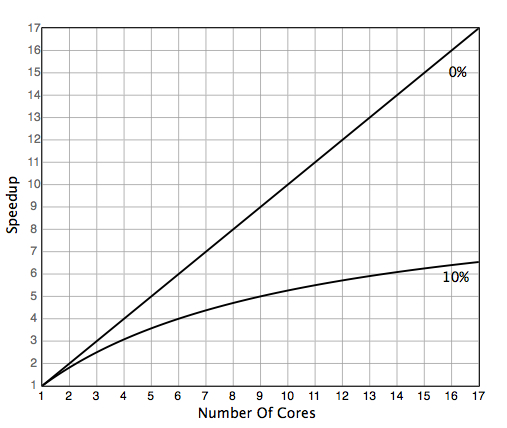
\includegraphics[width=0.75\textwidth]{Introduction/AmdahlsLaw10.jpg}
		\end{column}
	\end{columns}
\end{frame}


\begin{frame}<handout:0>{Amdahl's Law}
	20\% Synchronization
	\begin{columns}
		\begin{column}{0.25\textwidth}
		   $S(N) = \frac{1}{(1-P)+\frac{P}{N}}$\\
		   $P = 0.2$
		\end{column}
		\begin{column}{0.75\textwidth}
		     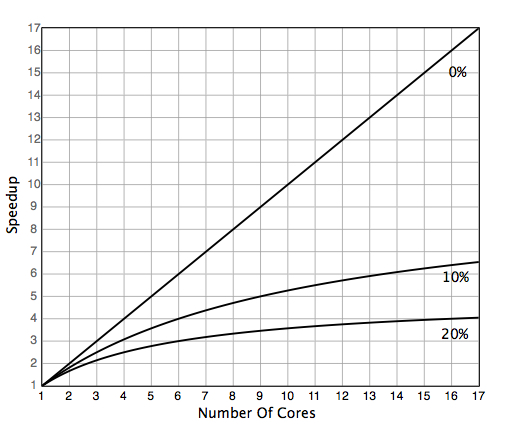
\includegraphics[width=0.75\textwidth]{Introduction/AmdahlsLaw20.jpg}
		\end{column}
	\end{columns}
\end{frame}


\begin{frame}{Amdahl's Law}
	90\% Synchronization
	\begin{columns}
		\begin{column}{0.25\textwidth}
		   $S(N) = \frac{1}{(1-P)+\frac{P}{N}}$\\
		   $P = 0.9$
		\end{column}
		\begin{column}{0.75\textwidth}
		     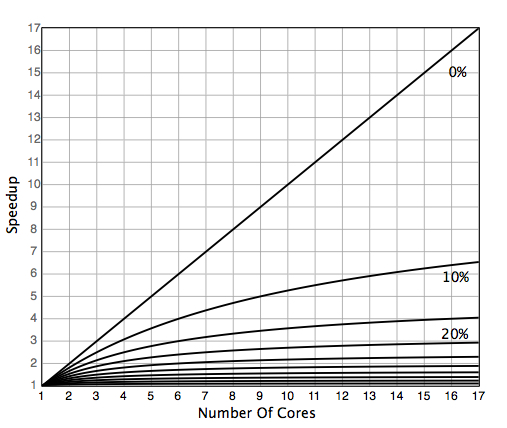
\includegraphics[width=0.75\textwidth]{Introduction/AmdahlsLaw90.jpg}
		\end{column}
	\end{columns}
\end{frame}


%=====================================================================================================
%=====================================================================================================
%=====================================================================================================


\part{Futures}


\begin{frame}{Outline Futures}
	\tableofcontents
\end{frame}


\section{Futures}


\subsection{Why Futures?}


\begin{frame}{Why Futures?}
	Why using futures?\\ \pause
	Aren't threads, mutex, atomics great?\\ \pause
	They are great tools "to shot yourself into the foot!"\\ \pause
	It is so easy 
	\begin{itemize}
		\item having race conditions
		\item having dead locks
		\item wasting CPU cycles through contention
	\end{itemize}
	\pause
	Do you program your application in assembly? \\ \pause
	Only if it absolute time critical.\\
	Then don't use tools from the level of assembly! 
\end{frame}


\subsection{Introduction}


\begin{frame}{Future Introduction}
    \begin{center}
    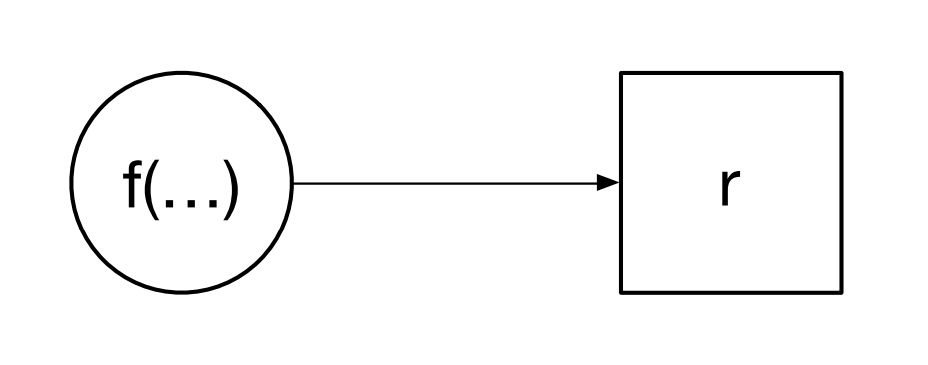
\includegraphics[width=0.6\textwidth]{Futures/future.jpg}   
    \end{center}
    \begin{itemize}
    \item<1->Futures provide a mechanism to separate a function from its result
    \item<2->After the function is called the result appears "magically" in the future
    \item<3->A future is a token to the result of a function
    \item<4->Added with C++11 
    \item<5->Futures, resp. promises where invented 1977/1978 by Daniel P. Friedman, David Wise, Henry Baker and Carl Hewitt
    \end{itemize}
\end{frame}


\subsection{C++ Standard - Futures}


\begin{frame}{C++ Standard - Futures}
    \lstinputlisting[language=C++,
                     linebackgroundcolor={%
                         \btLstHL<2>{1}%
                         \btLstHL<3>{8-11}%                         
                         \btLstHL<4>{13}%                         
                         \btLstHL<5>{15}%
                         \btLstHL<6>{16}%                         
                    }
    ]{Futures/future01.cpp}
    \pause\pause\pause\pause\pause
    \outputbox{42}  
\end{frame}


\subsubsection{Exceptions}


\begin{frame}{C++ Standard - Futures - Exceptions}
    \lstinputlisting[language=C++,
                     linebackgroundcolor={%
                         \btLstHL<2>{8-11}%
                         \btLstHL<3>{13}%
                         \btLstHL<4>{16,20}%                         
                         \btLstHL<5>{17-18}%
                         \btLstHL<6>{20-22}%
                    }
    ]{Futures/future02.cpp}
    \pause\pause\pause\pause
    \outputbox{Bad things happened: Vogons appeared!}
\end{frame}


\subsubsection{Deficiencies}


\begin{frame}{C++11/14 Future Deficiencies}
    \begin{itemize}
	    \item<2->No continuation –-- .then() \xmark $^\ast$
	    \item<3->No join –-- .when\_all() and  .when\_any() \xmark $^\ast$
	    \item<4->No split –-- continuation in different directions \xmark
	    \item<5->No cancellation (but can be modelled) \xmark
	    \item<6->No progress monitoring (except ready) \xmark
	    \item<7->No custom executor \xmark
	    \item<8->Blocks on destruction (may even blocks until termination of used thread) \xmark
	     \item<9->.get() has two problems:
	    \begin{enumerate}
    	    \item<10->One thread resource is consumed which increases contention and possibly causing a deadlock \xmark
    	    \item<11->Any subsequent non-dependent calculations on the task are also blocked \xmark
	    \end{enumerate}
	    \item<12->Don't behave as a regular type \xmark
    \end{itemize}
    \bigskip
    \pause$\ast$ Comes with C++17(TS)
\end{frame}


\subsection{Boost - Futures}


\subsubsection{Deficiencies}


\begin{frame}{Boost - Futures}
    \begin{itemize}
	    \item<2->Continuation –-- .then() \cmark
	    \item<2->Join –-- .when\_all() and .when\_any() \cmark
	    \item<3->No split –-- continuation in different directions \xmark
	    \item<3->No cancellation (but can be modelled) \xmark
	    \item<3->No progress monitoring (except ready) \xmark
	    \item<4->Custom executor \cmark
	    \item<5->Blocks on destruction (may even blocks until termination of used thread) \xmark
	    \item<5->.get() has two problems:
	    \begin{enumerate}
    	    \item<5->One thread resource is consumed which increases contention and possibly causing a deadlock \xmark
    	    \item<5->Any subsequent non-dependent calculations on the task are also blocked \xmark
	    \end{enumerate}
	    \item<5->Don't behave as a regular type \xmark
    \end{itemize}
\end{frame}


\subsubsection{Future Continuation}


\begin{frame}{Future Continuation}
    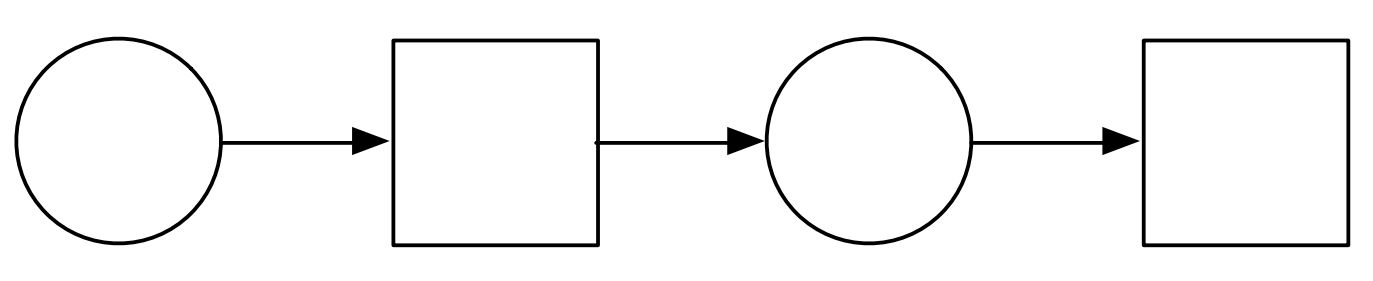
\includegraphics[width=\textwidth]{Futures/continuation.jpg}
\end{frame}


\begin{frame}{C++17(TS) / Boost - Continuation}
    \lstinputlisting[language=C++,
                     linebackgroundcolor={%
                         \btLstHL<2>{7}%
                         \btLstHL<3>{9-10}%                         
                         \btLstHL<4>{13}%
                    }
    ]{Futures/future03.cpp}
    \pause\pause\pause
    \outputbox{42}
\end{frame}


\subsubsection{Future Join}


\begin{frame}{Future Join}
    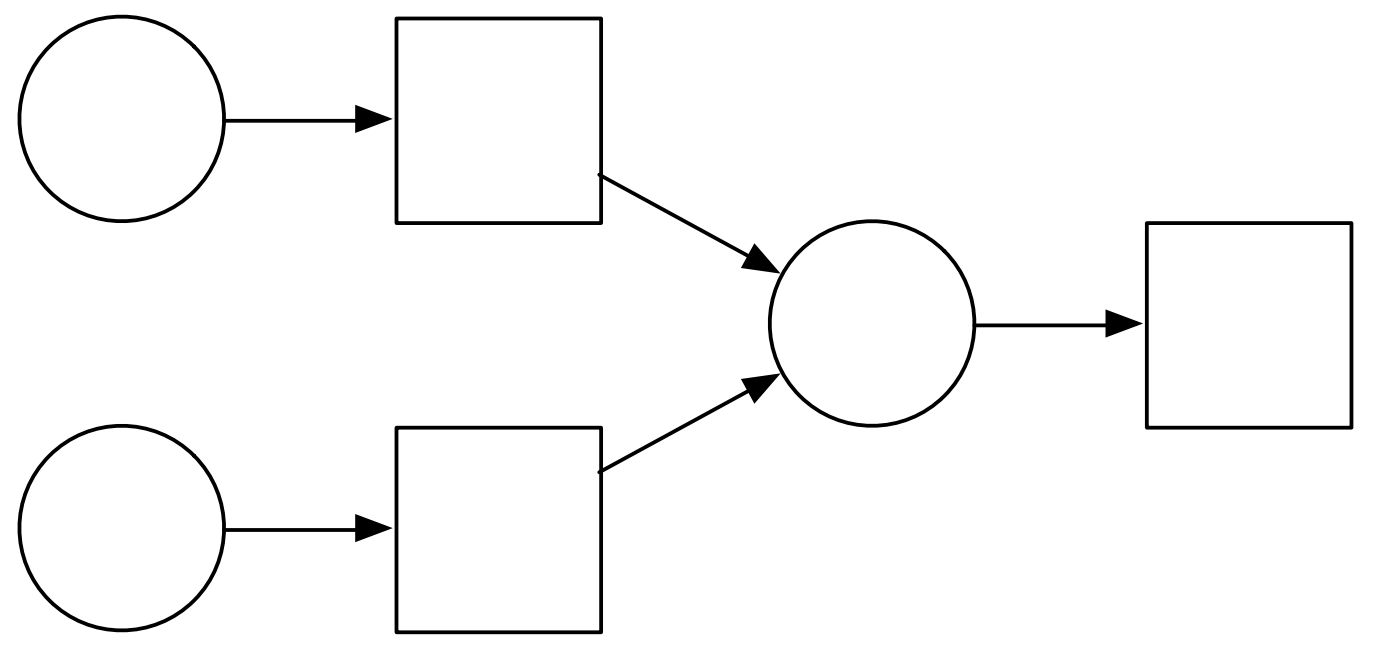
\includegraphics[width=\textwidth]{Futures/joins.jpg}
\end{frame}


\begin{frame}{C++17(TS) / Boost - Join}
    \lstinputlisting[language=C++,
                     linebackgroundcolor={%
                         \btLstHL<2>{7}%
                         \btLstHL<3>{8}%                         
                         \btLstHL<4>{10}%
                         \btLstHL<5>{11-14}%
                         \btLstHL<6>{17}%                
                    }
    ]{Futures/future04.cpp}
    \pause\pause\pause\pause\pause
    \outputbox{42}
\end{frame}


\begin{frame}{C++17(TS) / Boost - Join}
    \lstinputlisting[language=C++,
                     linebackgroundcolor={%
                         \btLstHL<1->{11}%                         
                    }
    ]{Futures/future04.cpp}
    What is the type of f?\linebreak
    \pause
    f is a future tuple of futures: \lstinline[style=CodeInTextStyle]|future<tuple<future<int>, future<int>>>|
\end{frame}


\subsection{stlab - Futures}

\begin{frame}{stlab - Futures}
	
\includegraphics[width=0.25\textwidth]{Futures/stlab_logo.png}
    \begin{center}	
        \textbf{stlab::future}\\
        Source: \url{https://github.com/stlab/libraries}\\
        Documentation: \url{http://www.stlab.cc/libraries}
    \end{center}
\end{frame}


\begin{frame}{stlab - Futures}
    \begin{itemize}
	    \item<2->Continuation –-- .then() \cmark
	    \item<3->Join –-- .when\_all() and .when\_any() \cmark
	    \item<4->Split –-- continuation in different directions \cmark
	    \item<5->Cancellation \cmark
	    \item<6->No progress monitoring (except ready), more planned \xmark
	    \item<7->Custom executor \cmark
	    \item<8->Do not block on destruction \cmark
	    \item<9->Behave as a regular type \cmark
	    \item<10->Additional dependencies:
		    \begin{itemize}
		    	\item C++14: boost (optional, variant)
		    	\item C++17: none
		    \end{itemize}
    \end{itemize}
\end{frame}


\begin{frame}{stlab::future}
    \lstinputlisting[language=C++,
                     linebackgroundcolor={%
                         \btLstHL<2>{1-2}%
                         \btLstHL<3>{6-9}%                         
                         \btLstHL<4>{11-14}%                         
                         \btLstHL<5>{15}%                         
                         \btLstHL<6>{10}%                         
                         \btLstHL<7>{18-20}%                  
                         \btLstHL<8>{22-23}%                         
                    }
    ]{Futures/future11.cpp}
    \pause\pause\pause\pause\pause\pause\pause
    \outputbox{42}  
\end{frame}


\begin{frame}{stlab::future - Exceptions}
    \lstinputlisting[language=C++,
                     linebackgroundcolor={%
                         \btLstHL<2>{7-10}%
                         \btLstHL<3>{11}%                         
                         \btLstHL<4>{14-15,19}%
                         \btLstHL<5>{21-23}%                         
                    }
    ]{Futures/future12.cpp}
    \pause\pause\pause\pause
    \outputbox{Bad things happened: Vogons appeared!}   
\end{frame}


\begin{frame}{stlab::future - Continuation}
    \lstinputlisting[language=C++,
                     linebackgroundcolor={%
                         \btLstHL<2>{6-7}%
                         \btLstHL<3>{9}%                         
                         \btLstHL<4>{11-13}%
                         \btLstHL<5>{10}%                          
                         \btLstHL<6>{11}%
                    }
    ]{Futures/future13.cpp}
    \pause\pause\pause\pause
    \outputbox{42}
\end{frame}


\subsubsection{Executors}


\begin{frame}{Executors}
	\begin{itemize}
		\item<2-> Executors are needed to customize where the task shall be executed
		\item<3-> Executors can be general thread pools, serial queues, main queues, dedicated task groups, etc.
	\end{itemize}
\end{frame}


\begin{frame}{stlab::future - Continuation with Custom Executor}
    \lstinputlisting[language=C++,
                     linebackgroundcolor={%
                         \btLstHL<2>{10-11}%
                         \btLstHL<3>{13-14}%                         
                         \btLstHL<4>{15}%                  
                    }
    ]{Futures/future14.cpp}    
\end{frame}


\begin{frame}{stlab::future - Custom Executor}
	\begin{itemize}
		\item<2-> In boost, executors derive from a common base class
		\item<3-> In stlab the executors must provide \lstinline[style=CodeInTextStyle]|
    template <typename F>
    void operator()(F f)|
    	\item<4-> Let's build exemplary a custom executor for the Qt GUI, that allows to perform updates in the Qt main event loop
	\end{itemize}
\end{frame}


\begin{frame}{stlab::future - Custom Executor - Qt}
    \lstinputlisting[language=C++,
                     linerange={1-7,9-11,26-27,40-47},
                     linebackgroundcolor={%
                         \btLstHL<2>{4}%
                         \btLstHL<3>{6}%                         
                         \btLstHL<4>{13-14}%
                         \btLstHL<5>{15-16}%
                         \btLstHL<6>{8-10}%
                    }
    ]{Futures/QtScheduler.cpp}
\end{frame}

\begin{frame}{stlab::future - Custom Executor - Qt cont. I}
    \lstinputlisting[language=C++,
                     linerange={1-27,40-41,47-47},
                     linebackgroundcolor={%
                         \btLstHL<1>{10}%
                         \btLstHL<2>{16-17}%
                         \btLstHL<3>{12,18}%                         
                         \btLstHL<4>{8,13,19}%
                         \btLstHL<5>{20}%
                         \btLstHL<6>{23}%
                         \btLstHL<7>{25}%
                    }
    ]{Futures/QtScheduler.cpp}
\end{frame}

\begin{frame}{stlab::future - Custom Executor - Qt cont. II}
    \lstinputlisting[language=C++,
                     linerange={1-5,10-11,25-39,40-47},
                     linebackgroundcolor={%
                         \btLstHL<1>{8}%
                         \btLstHL<2>{11}%                         
                         \btLstHL<3>{14}%
                         \btLstHL<4>{15,18}%
                         \btLstHL<5>{16,18,20}%
                         \btLstHL<6>{17, 26}%
                    }
    ]{Futures/QtScheduler.cpp}
\end{frame}

\subsubsection{Error Recovery}


\begin{frame}{stlab::future - Error Recovery}
    \lstinputlisting[language=C++,
   					   linerange={5-26},
                     linebackgroundcolor={%
                         \btLstHL<2>{2-5}%
                         \btLstHL<3>{6-9}%                         
                         \btLstHL<4>{11}%
                         \btLstHL<5>{12}%
                         \btLstHL<6>{13-16}%
                         \btLstHL<7>{17}% 
                         \btLstHL<8>{18}%            
                    }
    ]{Futures/future15.cpp}
    \pause\pause\pause\pause\pause\pause\pause\pause
    \outputbox{
Listen to Vogon poetry!\\
We have a problem!\\}
\end{frame}


\subsubsection{Join}


\begin{frame}{stlab::future - Join}
    \lstinputlisting[language=C++,
                     linebackgroundcolor={%
                         \btLstHL<2>{8}%
                         \btLstHL<3>{9}%                         
                         \btLstHL<4>{11}%
                         \btLstHL<5>{12}%
                         \btLstHL<6>{13}%
                         \btLstHL<7>{8,9,14}%
                         \btLstHL<8>{16-18}%
                         \btLstHL<9>{19}%
                    }
    ]{Futures/future16.cpp}
    \pause\pause\pause\pause\pause\pause\pause\pause
    \outputbox{42}
\end{frame}


\subsubsection{Splits}


\begin{frame}{future - Split}
    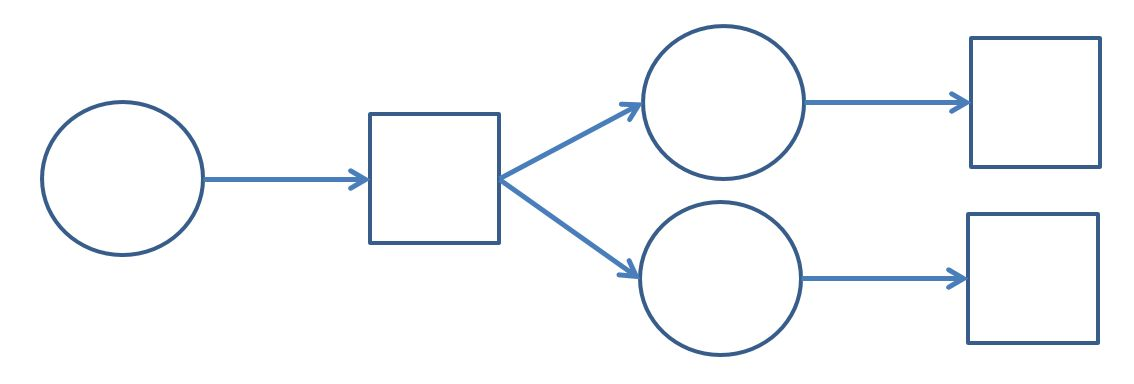
\includegraphics[width=\textwidth]{Futures/split.jpg}
\end{frame}


\begin{frame}{stlab::future - Split}
    \lstinputlisting[language=C++,
                     linebackgroundcolor={%
                         \btLstHL<2>{8}%
                         \btLstHL<3>{10-12}%                         
                         \btLstHL<4>{14-16}%
                         \btLstHL<5>{18-20}%
                    }
    ]{Futures/future17.cpp}
    \pause\pause\pause\pause
    \outputbox{
Tell the answer May the answer 42 Arthur Dent\\
42 shear up Marvin \pause $\textcolor{red}{\Rrightarrow}$ \textbf{\textcolor{red}{Race condition by using std::cout}}
}
\end{frame}


\subsection{Exercise 1}


\begin{frame}<handout:0>{Exercise 1}
  \begin{center}
  Demo Exercise 1
  \end{center}
\end{frame}


\begin{frame}{Exercise 1}
	Change the application in a way that
	\begin{itemize}
		\item using Start does not block the UI,
		\item it is possible to cancel the running operation,
		\item it is possible to restart it.
	\end{itemize}
\end{frame}


\begin{frame}{Conclusion}
	Futures are a great concept to structure the code so that it runs with minimal contention.\\
	\pause
	\medskip
	After a single execution the graph cannot be used any more.
\end{frame}


%=====================================================================================================
%=====================================================================================================
%=====================================================================================================


\part{Channels}


\begin{frame}{Outline Channels}
	\tableofcontents
\end{frame}


\section{Channel Motivation}

\begin{frame}{Channel Introduction}
    \begin{center}
    	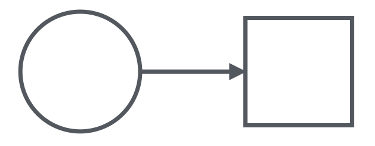
\includegraphics[width=0.5\textwidth]{Channels/simple_channel.png}
    \end{center}
    \begin{itemize}
    \item <2->Each change triggers a notification to the sink values
    \item <3->Channels allow the creation of persistent execution graphs    
    \item <4-> This is also known as reactive programming model
    \item <5-> First published by Tony Hoare 1978
    \end{itemize}
\end{frame}


\section{Channel - Stateless Process}

\begin{frame}{Channel - Stateless Process}
    \lstinputlisting[language=C++,
                linebackgroundcolor={%
							 \btLstHL<2>{1}%
							 \btLstHL<3>{2}%                         
							 \btLstHL<4>{5}%
							 \btLstHL<5>{6}%
							 \btLstHL<6>{7-8}%
							 \btLstHL<7>{10-11}%                         
							 \btLstHL<8>{13-15}%
							 \btLstHL<9>{16}%
							 \btLstHL<10>{18}%
							 \btLstHL<11>{20}%                         
							 }
    ]{Channels/channel01.cpp}
    \pause\pause\pause\pause\pause\pause\pause\pause\pause\pause\pause
    \outputbox{
    1\\
    2\\
    3\\}
\end{frame}


\subsection{Channel - Split}


\begin{frame}{Channel - Split}
    \begin{center}
    	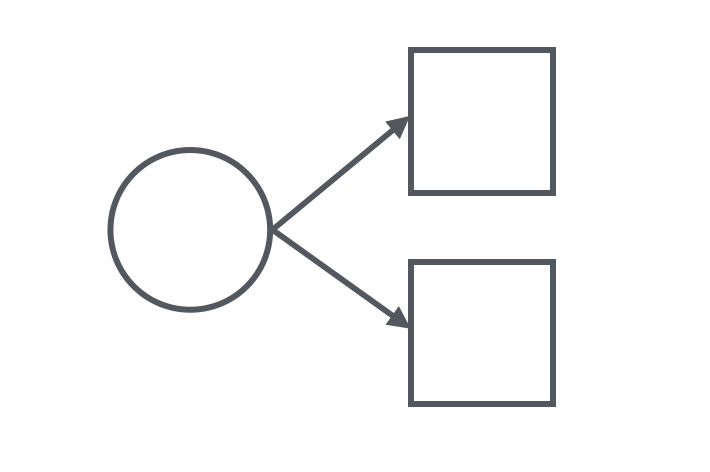
\includegraphics[width=0.75\textwidth]{Channels/simple_split.png}
    \end{center}
\end{frame}

\begin{frame}{Channel - Split Process}
    \lstinputlisting[language=C++,
    				  linerange={5-21},
                     linebackgroundcolor={%
                         \btLstHL<2>{3-5}%
                         \btLstHL<3>{7}%                         
                         \btLstHL<4>{8}%
                         \btLstHL<5>{10}%
						   \btLstHL<6>{11}%
                         \btLstHL<7>{13}%                         
                         \btLstHL<8>{15}% 
                    }
    ]{Channels/channel02.cpp}
    \pause\pause\pause\pause\pause\pause\pause\pause
    \outputbox{
	Process A 1 \\
	Process B 1 \\
	Process A 2 \\
	Process B 2 \\
	Process B 3 \\
	Process A 3 \\
	}
\end{frame}


\subsection{Channel - Join}


\begin{frame}{Channel - Join}
    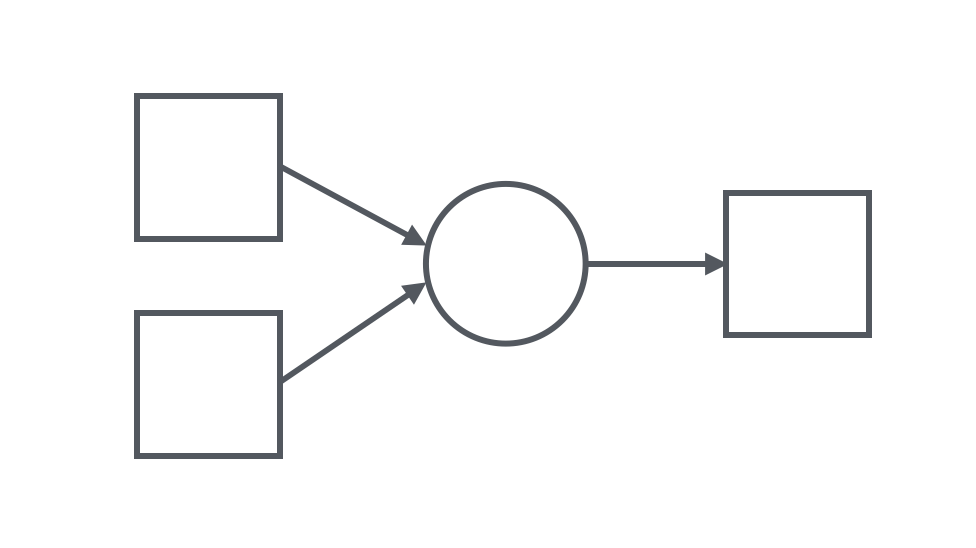
\includegraphics[width=\textwidth]{Channels/join.png}
\end{frame}

\begin{frame}{Channel - Joined Processes}
    \lstinputlisting[language=C++,
                     linerange={6-25},
                     linebackgroundcolor={%
                         \btLstHL<2>{6-7}%
                         \btLstHL<3>{9}%                         
                         \btLstHL<4>{11-12}%
                         \btLstHL<5>{14-15}%
						   \btLstHL<6>{17}%
                    }
    ]{Channels/channel03.cpp}
    \pause\pause\pause\pause\pause\pause
    \outputbox{
Process 1 3 \\
Process 2 5 \\
Process 4 6 \\
	}
\end{frame}


\begin{frame}{Channel operators}
	Beside \lstinline[style=CodeInTextStyle]|join()| there are:\\
	\begin{itemize}
		\item \lstinline[style=CodeInTextStyle]|zip()|The process takes the passed values in a round-robin manner, starting with the result from the first receiver.
		\item \lstinline[style=CodeInTextStyle]|merge()|The process takes the values in an arbitrary order. 
	\end{itemize}
\end{frame}


\subsection{Exercise 2}


\begin{frame}<handout:0>{Exercise 2}
  \begin{center}
  Demo Exercise 2
  \end{center}
\end{frame}


\begin{frame}{Exercise 2}
	Create a process chain with
	\begin{itemize}
	\item the inputs
		\begin{itemize}
			\item one \lstinline[style=CodeInTextStyle]|int| input
			\item one \lstinline[style=CodeInTextStyle]|std::string| input
			\item one \lstinline[style=CodeInTextStyle]|double| input
		\end{itemize}
	\item all inputs are joined to a process that concatenates all the results into a string and
	\item the result is split into
		\begin{itemize}
			\item one process that prints the result into console,
			\item one process that stores the result into a file
		\end{itemize}
	\item show with two value triplets, that the implementation works
	\item don't use any synchronization primitive
	\end{itemize}
\end{frame}

\begin{frame}{Conclusion}
	\begin{itemize}
		\item Stateless processes (from the point of view of the channel) have a 1:1 relationship from input to output
	\end{itemize}
\end{frame}


\section{Channel Stateful Process}


\begin{frame}{Channel Stateful Process - Motivation}
	\begin{itemize}
		\item Some problems need a processor with state
		\item Some problems have an n : m relationship from input to output
		\item The picture becomes more complicated with states:
		\begin{itemize}
			\item When to proceed?
			\item How to handle situations when less than expected values come downstream?
		\end{itemize}
	\end{itemize}
\end{frame}


\begin{frame}[fragile]{Channel - Stateful Process Signature }
    \lstinputlisting[language=C++
    ]{Channels/process_signature.cpp}
\end{frame}


\begin{frame}[fragile]{Stateful Process Signature - await}
    \lstinputlisting[language=C++,
                     linebackgroundcolor={%
                         \btLstHL<1>{8}%
                    }
    ]{Channels/process_signature.cpp}
The \lstinline[style=CodeInTextStyle]|await| method is called on the process whenever a new value was received from upstream. The type T stands here for any semi regular or move-only type. The number of arguments depends on the number of attached upstream sender. Potential state changes from awaitable to yieldable should happen while this method is invoked.
\end{frame}


\begin{frame}[fragile]{Stateful Process Signature - yield}
    \lstinputlisting[language=C++,
                     linebackgroundcolor={%
                         \btLstHL<1>{10}%
                    }
    ]{Channels/process_signature.cpp}
The \lstinline[style=CodeInTextStyle]|yield| method is called on the process whenever the \lstinline[style=CodeInTextStyle]|process_state_scheduled.first| is \lstinline[style=CodeInTextStyle]|process_state::yield| or a timeout was provided with the recent call to \lstinline[style=CodeInTextStyle]|state()| and that has elapsed.
\end{frame}


\begin{frame}[fragile]{Stateful Process Signature - state}
    \lstinputlisting[language=C++,
                     linebackgroundcolor={%
                         \btLstHL<1>{3-4,12}%
                    }
    ]{Channels/process_signature.cpp}
This method must return the current state of the process.  Typical return values are \lstinline[style=CodeInTextStyle]|await_forever| and \lstinline[style=CodeInTextStyle]|yield_immediate|. By explicit using the second part of the return type, one can set a possible timeout. Subsequent calls \textit{without} an intermittent \lstinline[style=CodeInTextStyle]|await(), close(), or yield()| must return the same values. Otherwise the result is undefined.
\end{frame}


\begin{frame}[fragile]{Stateful Process Signature - close}
    \lstinputlisting[language=C++,
                     linebackgroundcolor={%
                         \btLstHL<1>{14}%
                    }
    ]{Channels/process_signature.cpp}
The optional \lstinline[style=CodeInTextStyle]|close()| method is called on the process whenever the process state is \lstinline[style=CodeInTextStyle]|await_forever| and the incoming queue went dry. As well it is called when an exception is thrown while calling \lstinline[style=CodeInTextStyle]|await()| or \lstinline[style=CodeInTextStyle]|yield()| and no \lstinline[style=CodeInTextStyle]|set_error()| is available.
\end{frame}


\begin{frame}[fragile]{Stateful Process Signature - set\_error}
    \lstinputlisting[language=C++,
                     linebackgroundcolor={%
                         \btLstHL<1>{16}%
                    }
    ]{Channels/process_signature.cpp}
The method \lstinline[style=CodeInTextStyle]|set_error()| is optional. It is called if either on calling \lstinline[style=CodeInTextStyle]|await()| or \lstinline[style=CodeInTextStyle]|yield()| an exception was thrown. The pointer of the caught exception is passed. In case that the process does not provide this method, \lstinline[style=CodeInTextStyle]|close()| is called instead of.
\end{frame}


\begin{frame}{Channel - Stateful Process Example}
    \lstinputlisting[language=C++,
  					  linerange={1-4, 5-7, 26, 27-43},
                     linebackgroundcolor={%
                         \btLstHL<2>{11-13}%
                         \btLstHL<3>{15-16}%
                         \btLstHL<4>{18}%
                         \btLstHL<5>{20-24}%
                    }
    ]{Channels/channel04.cpp}
\end{frame}


\begin{frame}{Channel - Stateful Process Example cont.}
    \lstinputlisting[language=C++,
  					  linerange={6-28,33-35,38-43},
                     linebackgroundcolor={%
                         \btLstHL<1>{1}%
                         \btLstHL<2>{3}%
                         \btLstHL<3>{4,20}%
                         \btLstHL<4>{6-11}%
                         \btLstHL<5>{13-18}%
                         \btLstHL<6>{7,8,29}%
                    }
    ]{Channels/channel04.cpp}
\end{frame}


\subsection{Exercise 3}


\begin{frame}<handout:0>{Exercise 3}
  \begin{center}
  Demo Exercise 3
  \end{center}
\end{frame}


\begin{frame}{Exercise 3}
	\hfill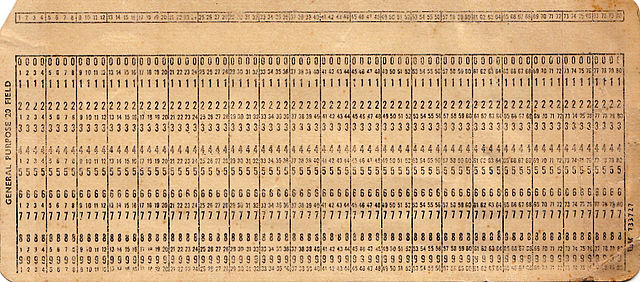
\includegraphics[scale=0.5]{Channels/640px-Punched_Card.jpg}\footnotemark\hspace*{\fill}
	\footnotetext{{\tiny By Ventriloquist - Own work, CC BY-SA 3.0, \url{https://en.wikipedia.org/w/index.php?curid=32753387}}}
	\\
	\pause
	A process which inputs cards of eighty characters and outputs their text, tightly packed into lines of 125 characters each.
	\begin{itemize}
		\item Write one process - unpack - that collect 80 chars in a bunch and yields them one after the other
		\item Write one process - pack - that packs 125 chars and yields them.
		\item Concatenate unpack - pack as a process chain.
		\item In a next step write one process - filter - that drops all newlines from the stream
		\item Concatenate now unpack - filter - pack as a process chain.
	\end{itemize}
\end{frame}


\part{Code Transformation}


\section{Process Analysis}


\begin{frame}{Process Analysis}
	\begin{itemize}
		\item Are there performance or usability problems?
		\item Identify the overall critical part
		\item Disassemble this part into individual processes
		\item Chain the processes with futures or channels 
	\end{itemize}
\end{frame}


\subsection{Example Use Cases}


\begin{frame}{Use case example I}
	Problem within our mammography application:
	\begin{itemize}
		\item<2-> Medical device shall open every case in $<1$ s
		\item<3-> Loading of patient data and first images takes about 0.6 s
		\item<4-> Reading of additional data structures (CAD\footnotemark reports) may take more than 0.4 s
		\item<5-> Direct access to any CAD report might be required
		\item<6-> If the user skips this case and advances to the next one, outstanding load operations should be cancelled or at least be ignored
		\only<4->\footnotetext{\textbf{C}omputer \textbf{A}ided \textbf{D}etection}
	\end{itemize}
\end{frame}


\subsection{Exercise 4}


\begin{frame}<handout:0>{Exercise 2}
  \begin{center}
  Demo Exercise 4
  \end{center}
\end{frame}


\begin{frame}{Exercise 4}
  Improve the application that the UI is always responsible\\
  \begin{itemize}
    \item On Reset the reports are newly read
    \item If one presses 1 or 2 while the reset is running, the reports shall be displayed as soon as they become available.
  \end{itemize}
\end{frame}


\part{Next Steps?}


\section{Next Steps?}

\begin{frame}{Next Steps?}
	High level concurrency sessions at ACCU 2017:\\
	\begin{itemize}
	  \item Thinking Outside the Synchronisation Quadrant by Kevlin Henney (Wed.)
		\item Coroutines in Python by Robert Smallshire (Thur.)
		\item Coroutines in C++ by Dominic Robinson (Fr.)
		\item Concurrency / Coroutines by Anthony Williams (Sat.)
	\end{itemize}
		
\end{frame}

%=====================================================================================================
%=====================================================================================================
%=====================================================================================================


\part{Bonus Material}


\section{Synchronization}

\begin{frame}{Synchronization Motivation}
	Why do we have to synchronize?\\ 
	\pause
	\textit{Because we have to ensure sequential consistency.}\\
	\pause
	What synchronization mechanism do you know?\\
	\pause
	\textit{
		\begin{itemize}
			\item<4-> Synchronization primitives (mutex, atomic, memory fence, ...)
			\item<5-> Guaranteed sequential access
		\end{itemize}
	}
\end{frame}


\section{Synchronization with Mutex}


\begin{frame}{Synchronization with Mutex}
    \lstinputlisting[language=C++,
                     linerange={7-35},
                     linebackgroundcolor={%
                         \btLstHL<2>{1-2}%
                         \btLstHL<3>{4-5}%
                         \btLstHL<4>{7-12}%
                         \btLstHL<5>{14-17}%
                         \btLstHL<6>{21}%
                         \btLstHL<7>{22-24}% 
                         \btLstHL<9>{10}% 
                         \btLstHL<10>{9}%                                             
                    }
    ]{Synchronization/mutex01.cpp}
    \pause\pause\pause\pause\pause\pause\pause
    Where are the problems in the code?
\end{frame}


\begin{frame}{Synchronization with Mutex}
	Mutex - What would be a better name for it?\\
	\pause
	\medskip 
	\textit{Bottleneck!}\footnotemark
	\only<2->{\footnotetext{Kevlin Henney, NDC London 2017}}
\end{frame}


\section{Synchronization without Mutex}

\begin{frame}{Synchronization without Mutex}
	How can the code be transformed into something without a mutex in the client code?\\
	\pause
	What is needed to perform that transformation? Which tools do we have in our tool box?
\end{frame}


\begin{frame}{Synchronization without Mutex}
    \lstinputlisting[language=C++,
                     linebackgroundcolor={%
                     	   \btLstHL<2>{1-2}%
                         \btLstHL<3>{4}%
                         \btLstHL<4>{5}%
                         \btLstHL<5>{7-13}%
                         \btLstHL<6>{15-20}%                                  
                    }
    ]{Synchronization/mutex02.cpp}
\end{frame}


\begin{frame}{Synchronization Epilogue}
	\begin{center}
  		So we try to avoid mutexes wherever it is possible.
  	\end{center}
\end{frame}


\begin{frame}{Synchronization Epilogue}
	\begin{center}
		All computer wait at the same speed
	\end{center}
\end{frame}



\begin{frame}{Use case example II}
	Image Preparation Pipeline
	\begin{itemize}
		\item A medial device shall display multi-frame image data sets
		\item Each incoming data set is JPEG 2000 compressed
		\item The slices must be decompressed and then compressed in FELICS\footnote{Special compression algorithm for 16bit grayscale images }  format for fast decompression and display
		\item Reading and writing to disk takes a reasonable amount of time
	\end{itemize}
\end{frame}


%=====================================================================================================
%=====================================================================================================
%=====================================================================================================

\part{Is there more?}

\section{Reference}

\subsection{Reference}

\begin{frame}{Reference}
    \begin{itemize}
    	\item Concurrency library \url{https://github.com/stlab/libraries}
    	\item Documentation \url{http://www.stlab.cc/libraries}
    	\item Communicating Sequential Processes by C. A. R. Hoare \url{http://usingcsp.com/cspbook.pdf}
    	\item The Theory and Practice of Concurrency by A.W. Roscoe\url{http://www.cs.ox.ac.uk/people/bill.roscoe/publications/68b.pdf}
    \end{itemize}
\end{frame}

\begin{frame}{Further reading I}
    Software Principles and Algorithms
    \begin{itemize}
        \item Elements of Programming by Alexander Stepanov, Paul McJones, Addison Wesley
        \item From Mathematics to Generic Programming by Alexander Stepanov, Daniel Rose, Addison Wesley
    \end{itemize}
\end{frame}


\begin{frame}{Further reading II}
    Concurrency and Parallelism
    \begin{itemize}
        \item HPX \url{http://stellar-group.org/libraries/hpx/}
        \item C++CSP \url{https://www.cs.kent.ac.uk/projects/ofa/c++csp}
        \item CAF\_C++ Actor Framework \url{http://actor-framework.org/}
        \item C++ Concurrency In Action by Anthony Williams, Manning (2nd edition coming soon)
    \end{itemize}
\end{frame}


\subsection{Further viewing}

\begin{frame}{Further viewing}
    \begin{itemize}
        \item Goals for better code by Sean Parent: \url{http://sean-parent.stlab.cc/papers-and-presentations}
        \item Goals for better code by Sean Parent: Concurrency: \url{https://youtu.be/au0xX4h8SCI?t=16354}
        \item Thinking Outside the Synchronization Quadrant by Kevlin Henney: \url{https://vimeo.com/205806162}
    \end{itemize}
\end{frame}


\section{Acknowledgement}

\begin{frame}{Acknowledgement}
	\begin{itemize}
		\item My family, who gave me the freedom to develop over months the library, prepare this tutorial and let me travel to the ACCU.
		\item Sean Parent, who taught me over time lots about concurrency and abstraction. He gave me the permission to use whatever I needed from his presentations for my own.
		\item My company MeVis Medical Solutions AG, that released me from work during the ACCU.
	\end{itemize}
\end{frame}


\section{Contact}

\begin{frame}{Contact}
	\begin{itemize}
		\item Mail: felix@petriconi.net
		\item Web: \url{https://petriconi.net}
		\item Twitter: @FelixPetriconi	 
	\end{itemize}
\end{frame}



\end{document}



% MAC installation guideline
% brew install gcc-6
% brew install freetype
% install xQuarz

% Linux installation guideline
% install gcc 6 
% sudo apt-get install libx11-dev
% sudo add-apt-repository ppa:no1wantdthisname/ppa
% sudo apt update && sudo apt install libfreetype6 libfreetype6-dev
% sudo apt-get install libxft-dev